% Mirror: https://github.com/SIGma-UIUC/presentation-format
% --------------------------------------------------------------------
% This is a simple Beamer document that uses beamerthemesigma.sty
% Reading the comments should help you create a presentation even if
% you've never used Beamer before.
% --------------------------------------------------------------------

% Set our document class to Beamer
\documentclass[aspectratio=169]{beamer}

% Some packages for nice font encodings in the final PDF
\usepackage[utf8]{inputenc}
\usepackage[T1]{fontenc}

% From Jeff E
\usepackage{algo}

% Some more macros
\usepackage{sigmastyle}

% Citations
\usepackage{cite}

% To insert images
\usepackage{graphicx}

% Useful packages from the AMS
\usepackage{amsmath,amssymb,amsthm}

\usepackage{soul}

% Package for code highlighting
\usepackage{minted}
\setminted{linenos=true, breaklines=true, breakanywhere=true, style=default}
\usemintedstyle{monokai}

% Set a title
\title{Ramsey's Theorem}

% Whoever worked on the presentation:
\author{Parth Deshmukh}

% Date looks ugly, so leave blank
\date{}


% Use the SIGma theme for this Beamer presentation
\usetheme{sigma}
% --------------------------------------------------------------------

% Begin document
\begin{document}

% Beamer calls each slide a "frame", defined within the environment:
% \begin{frame}
%   <frame content here>
% \end{frame}

% This frame is just the title.
\begin{frame}
\titlepage
\end{frame}

% A frame with the table of contents.
% This frame's title is "Outline".
\begin{frame}{Outline}
  \tableofcontents
\end{frame}

% Start a section: *sections* (subsections, etc.) are what show up in the TOC.
\section{Friends and strangers}
% Section pages can be printed thus:
\frame{\sectionpage}
% There's a way to automate this, see:
% https://tex.stackexchange.com/questions/178800/creating-sections-each-with-title-pages-in-beamers-slides/178803

\subsection{Setup} %% for table of contents
\begin{frame}{Six people walk into a party...}
    
    \begin{itemize}
        \item We can prove that there's a group of three people who all know each other or all don't know each other. \pause
        \item How do we represent this? \pause
        \item {\color{sigma@alertred} Coloring the edges of graphs!}
    \end{itemize}

    
\end{frame}

\begin{frame}{Into graph land}
    We represent each person as a vertex, and connect two people with a \textcolor{sigma@alertred}{red edge} if they know each other, and a \textcolor{sigma@mainblue}{blue edge} if they don't.
    
    \begin{figure}
        \centering
        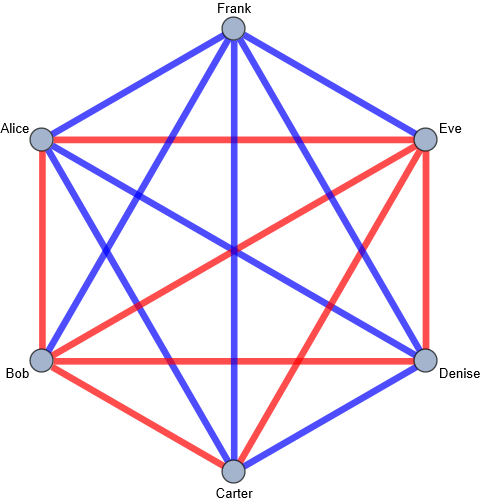
\includegraphics[width=0.4\columnwidth]{images/exampler33k6.png}
        \caption{Our party - poor Frank doesn't know anyone :(}
    \end{figure}
\end{frame}

\subsection{Theorem and proof} %% for table of contents
\begin{frame}{Friends and strangers}
    \begin{theorem}
        In a group of six people, there are either three people who all know each other or three people who all don't know each other.
    \end{theorem} \pause
    \vspace{20pt}
    Formally:
    \begin{theorem}
        If we color the edges of a complete graph $K_6$ with two colors, there will be at least one monochromatic triangle as a subgraph.
    \end{theorem}
\end{frame}

\begin{frame}{Proof of the theorem of friends and strangers}
    We will prove by contradiction. Our goal is to color a $K_6$ so it has no monochromatic triangle. Let's focus on one vertex, highlighted in green:
    \begin{figure}
        \centering
        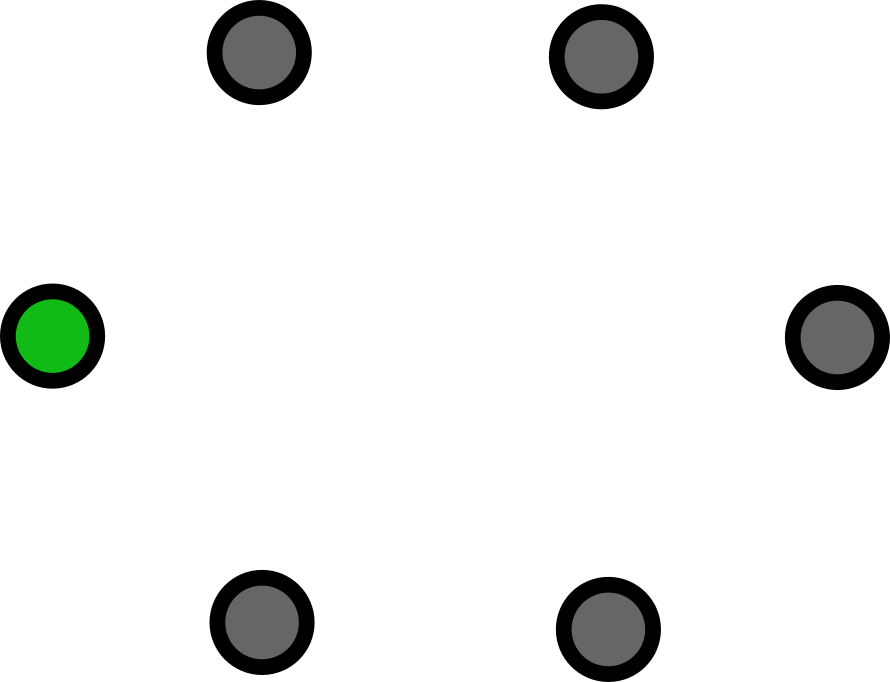
\includegraphics[width=0.5\columnwidth]{images/step1.png}
    \end{figure}
\end{frame}

\begin{frame}{Proof of the theorem of friends and strangers}
    By the pigeonhole principle, at least 3 of this vertex's edges must be red:
    \begin{figure}
        \centering
        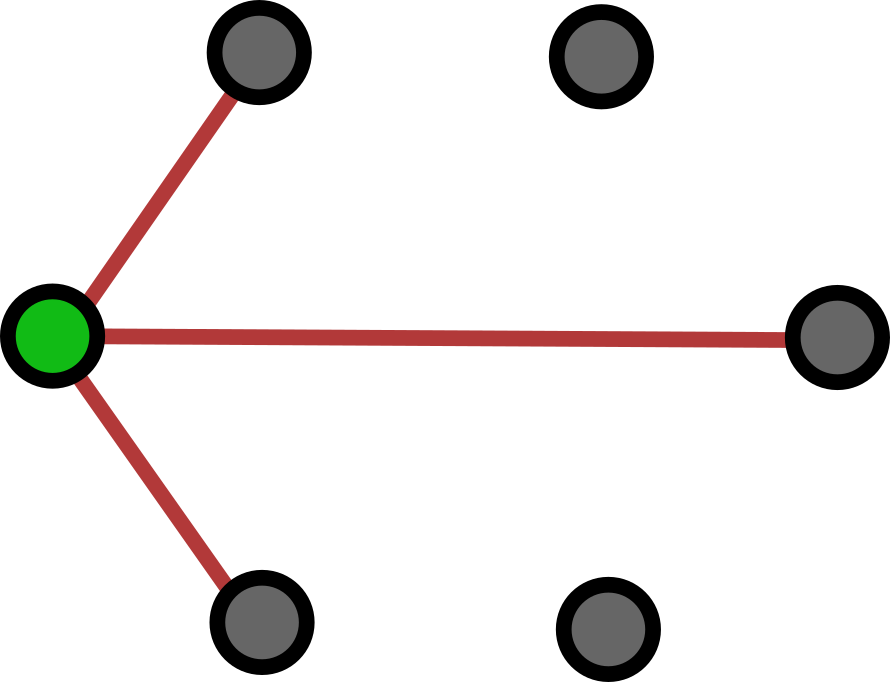
\includegraphics[width=0.5\columnwidth]{images/step2.png}
    \end{figure}
    If no such vertex exists, then every vertex has at least 3 blue edges; swap blue and red.
\end{frame}

\begin{frame}{Proof of the theorem of friends and strangers}
    Now we need to connect those three neighbors. We can't connect them with a red edge, because that'd make a red triangle!
    \begin{figure}
        \centering
        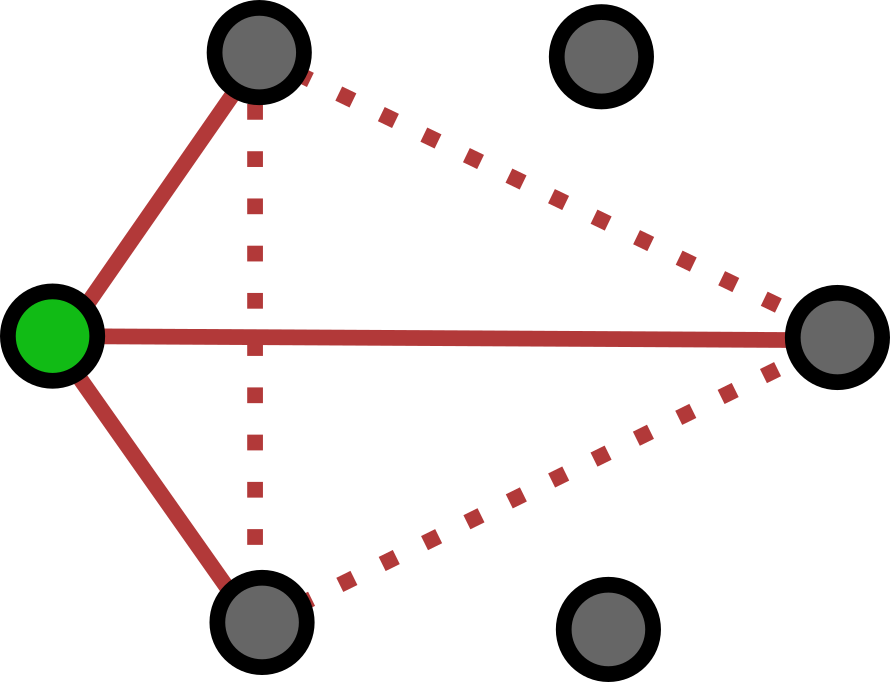
\includegraphics[width=0.5\columnwidth]{images/step3.png}
    \end{figure}
\end{frame}

\begin{frame}{Proof of the theorem of friends and strangers}
    So we have to connect them in blue, making a blue triangle. Thus we can't avoid making a monochromatic triangle, proving the theorem.
    \begin{figure}
        \centering
        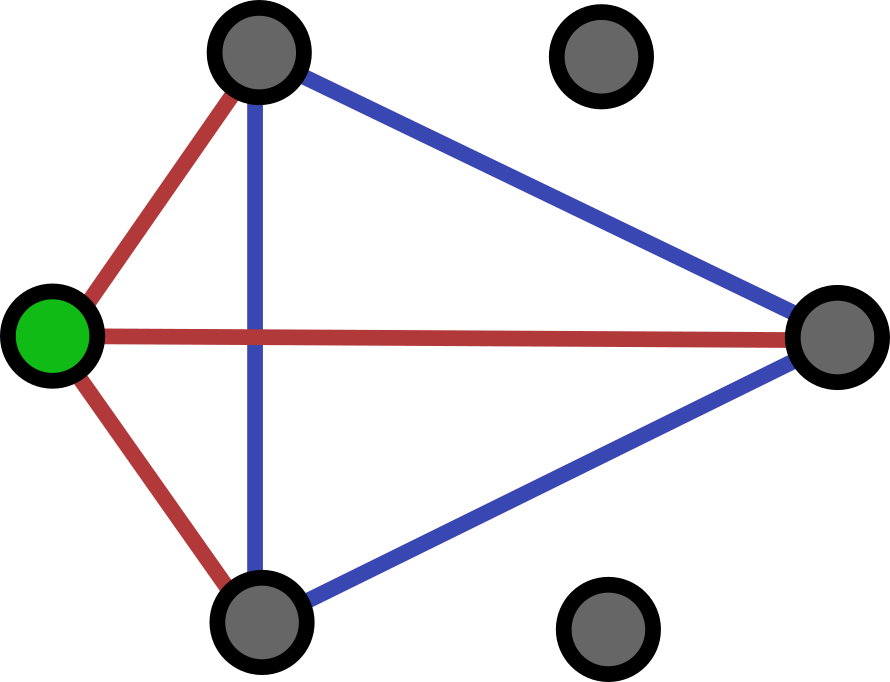
\includegraphics[width=0.5\columnwidth]{images/step4.png}
    \end{figure}
\end{frame}

\begin{frame}{Different numbers of people}
    \begin{itemize}
        \item What if we have more than six people? \pause
        \item If we have six or more people, this property holds because there's a copy of $K_6$ inside our representative graph $K_n, n>=6$.
    \end{itemize}
    \begin{figure}
        \centering
        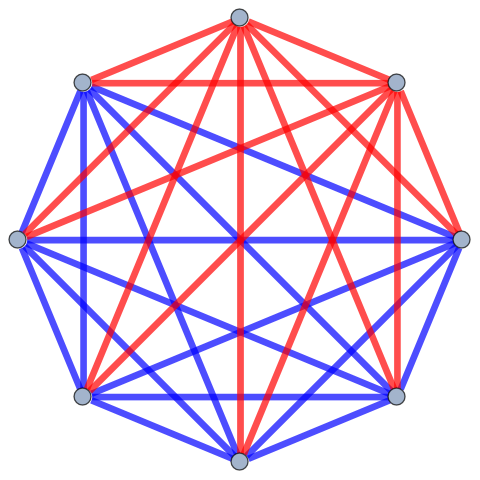
\includegraphics[width=0.3\textwidth]{images/r8example.png}
        \caption{The subgraph marked by the blue edges is a copy of $K_6$.}
    \end{figure}
\end{frame}

\begin{frame}{Different numbers of people}
    \begin{itemize}
        \item What if we have five people? \pause
        \item Looking at $K_5$, this property no longer holds:
    \end{itemize}
    \begin{figure}
        \centering
        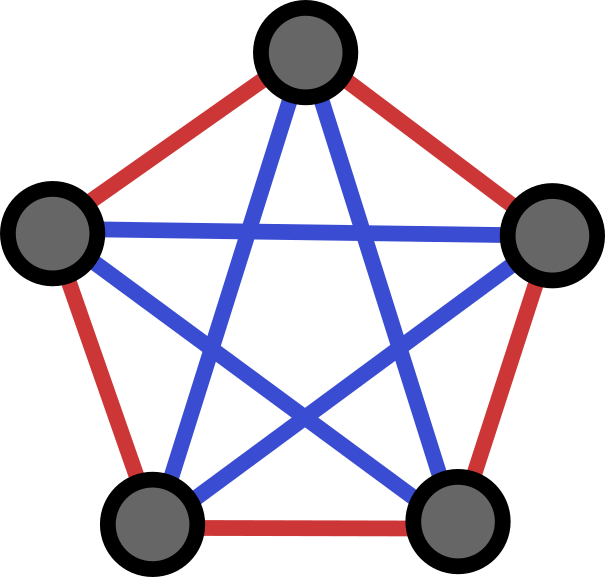
\includegraphics[width=0.3\columnwidth]{images/k5.png}
        \caption{Each set of colored edges is a cycle of 5 elements, so no triangles!}
    \end{figure}
\end{frame}

\begin{frame}{Different numbers of people}
    Thus, the statement should really be ``six \textit{or more} people.'' So this theorem really gives us a \textit{threshold} of some sort. What is this threshold?
\end{frame}
% Another frame:
% \begin{frame}
%   % Alternate syntax for frame titles
%   \frametitle{There Is No Largest Prime Number}
%   % Frames can have subtitles:
%   \framesubtitle{The proof uses \textit{reductio ad absurdum}.}
%   % Some frame content:
%   \begin{theorem}
%     There is no largest prime number.
%   \end{theorem}
%   \begin{enumerate}
%     % We do some interesting stuff with the items to make them appear
%     % on sequential slides. See the PDF for how this turns out. The
%     % first item is set to alert on the first slide in red.
%     \item<1-| alert@1> Suppose $p$ were the largest prime number.
%     \item<2-> Let $q$ be the product of the first $p$ primes.
%     \item<3-> Then $q+1$ is not divisible by any of them.
%     \item<4-> But $q + 1$ is greater than $1$, thus divisible by some prime
%     number not in the first $p$ numbers.
%     \item<5-> There exists a prime larger than $p$.
%   \end{enumerate}
% \end{frame}


\section{Ramsey's Theorem}
\frame{\sectionpage}

\begin{frame}{The full theorem}
    \begin{theorem}
        Let integers $k, l > 2$. Then there exists a minimum positive integer $R(k, l)$ so that if we color the edges of a complete graph with $R(k, l)$ vertices red or blue, there is either a monochromatic red clique of $k$ vertices or blue clique of $l$ vertices. \cite{Bona06}
    \end{theorem}
    \begin{itemize}
        \item A ``clique'' is a complete subgraph.
        \item Our theorem of friends and strangers is really proving $R(3,3) = 6.$
    \end{itemize}
    
\end{frame}

% Similar for subsections:
% \subsection{A subsection, Wow}
% And their pages:
% \frame{\subsectionpage}

% \begin{frame}{Side by Side}
%     
\includegraphics[width=0.25\textwidth]{sigma.png}\hspace{0.4\textwidth}
%     
\includegraphics[width=0.25\textwidth]{sigma.png}
% \end{frame}
\begin{frame}{Proof sketch}
    \begin{itemize}
        \item The proof of Ramsey's theorem uses induction.
        \item Note that $R(k,l) = R(l,k)$. We also have $R(k, 2) = k$ for the base cases.
        \item The inductive step is:
    \end{itemize}
    \[
        R(k, l) \leq R(k, l-1) + R(k-1, l)
    \]
\end{frame}

\section{Calculating the Ramsey numbers}
\frame{\sectionpage}

\subsection{Complexity} % for table of contents
\begin{frame}{Just use a computer, right?}
    \begin{itemize}
        \item Unfortunately, the time complexity grows far too fast. 
        \item Suppose we want to check if $R(5, 5) = N.$ 
        \item A naive program would look like:
    \end{itemize}
    \begin{algo}
        \underline{\textsc{Ramsey}(5, 5, N):}\+
    \\      \textbf{for} every coloring $C$ of $K_N$:\+
    \\          \textbf{if} $C$ does not contain a monochromatic 5-clique:\+
    \\              \textbf{output} \textsc{NO} and the coloring $C$\-\-
    \\      \textbf{output} \textsc{YES}
    \end{algo}
    There might be better algorithms\cite{site:stackexchange}, but there's not a lot of work on them; nothing seems to be fixing the time complexity just yet.
\end{frame}

\begin{frame}{Time complexity}
    \begin{itemize}
        \item The graph $K_N$ has $N \choose 2$ edges. Coloring each edge involves a choice of one of two colors, so the total number of colorings is $2^{N \choose 2}$. \pause
        \item Naive $O\pqty{2^{N \choose 2}}$ time complexity! For comparison, here's it against $O\pqty{N!}$ and $O\pqty{2^N}:$ \pause
    \end{itemize}
    \begin{figure}
        \centering
        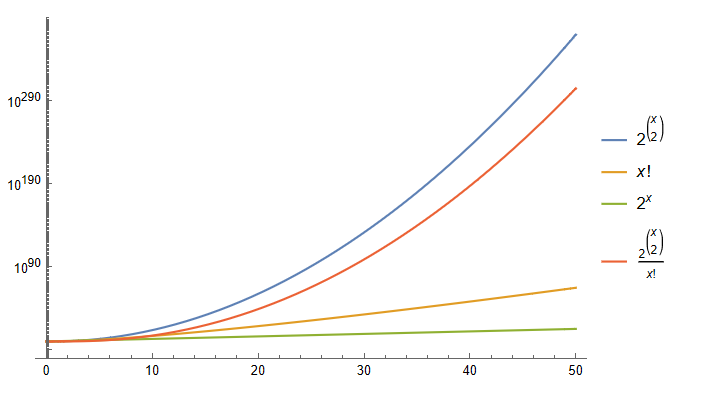
\includegraphics[width=0.6\columnwidth]{images/complexitycompairson.png} % \columnwidth == \textwidth it seems
        \caption{$43 \leq R(5,5) \leq 48$}
    \end{figure}
\end{frame}

\subsection{Bounds} % for table of contents
\begin{frame}{Bounds}
\begin{itemize}
    \item We can at least set bounds on Ramsey numbers. \pause
    \item  Upper bound: \cite[13.6, 13.7]{Bona06}
    \begin{gather*}
        R(k, l) \leq {k+l-2 \choose k-1} \\
        R(k, k) \leq {2k - 2 \choose k -1} \leq 4^{k-1}
    \end{gather*} \pause
    \item  Lower bound: \cite[15.5]{Bona06}
    \[
    (\sqrt{2})^k \leq R(k,k) \leq 4^{k-1}
    \]
    \item The proof for the lower bound uses the \textcolor{sigma@mainblue}{\emph{probabilistic method}}.
\end{itemize}
\end{frame}

\section{The wide world of Ramsey theory}
\frame{\sectionpage}

\begin{frame}{Ramsey-type theorems}
    \textit{Ramsey Theory}\cite[1.3]{Graham} lays out the ``Super Six:''
    \begin{itemize}
        \item Ramsey's theorem \pause
        \item Van der Waerden's theorem: if you color the positive integers, there is a monochromatic arithmetic progression \pause
        \item Schur's theorem: if you color the positive integers, there are three integers $x,y,z$ of the same color such that $x + y = z$ \pause
        \item Rado's theorem: There exist monochromatic solutions to integer linear equations \pause
        \item Hales-Jewett theorem: Color an n-dimensional cube, there always exists a monochromatic line of points \pause
        \item Graham-Leeb-Rothschild theorem: Hales-Jewett theorem for subcubes instead of lines
    \end{itemize}
\end{frame}

\begin{frame}{General vibes}
    \begin{itemize}
        \item Finding ordered substructures inside partitions of sets \pause
        \item Finding bounds for when those substructures pop up
        \begin{itemize} % not the best way to do sublists, but I'm too lazy to define a command just for this
            \item Van der Waerden and Schur are concerned with coloring the first $N$ integers
        \end{itemize} \pause 
        \item Those bounds tend to blow up \textit{really} quickly and are even harder to compute \pause
        \begin{itemize}
            \item The proof that S(5) = 161 took 2 petabytes of space!
            \item \url{https://www.cs.utexas.edu/~marijn/Schur/}
        \end{itemize}
    \end{itemize}
\end{frame}

% Asking questions is fun but we should answer some first
\begin{frame}{}
      \begin{center}
    {\color{sigma@mainblue} \LARGE Questions?}
  \end{center}
\end{frame}

\font\eightss=cmssq8
\font\eightssi=cmssqi8
\newcommand\quoteAuthorDate[3]{\begingroup
  \baselineskip 10pt
  \parfillskip 0pt
  \interlinepenalty 10000 % not needed in example
  \leftskip 0pt plus 40pc minus \parindent
  \let\rm=\eightss
  \let\sl=\eightssi
  \everypar{\sl}#1\par
  \nobreak\smallskip
  \noindent\rm--- #2\unskip\enspace(#3)\par
  \endgroup}
% If someone can figure out how to horizontally center this and make the text bigger that'd be cool
\begin{frame}
    \begin{center}
        \item \quoteAuthorDate{Aliens invade the earth and threaten to obliterate it in a year’s time unless human beings can find the Ramsey number for red five and blue five. We could marshal the world’s best minds and fastest computers, and within a year we could probably calculate the value. If the aliens demanded the Ramsey number for red six and blue six, however, we would have no choice but to launch a preemptive attack.}{PAUL ERDOS}{\cite{Graham}}
    \end{center}
\end{frame}

% Remove this slide if you came up with all the material yourself
\begin{frame}{Bibliography}
    \bibliography{refs}
    \bibliographystyle{alpha}
\end{frame}

\end{document}